\documentclass[border=10pt]{standalone}
\usepackage{tikz}\usepackage{amsmath}\usetikzlibrary{calc,arrows.meta}
\begin{document}
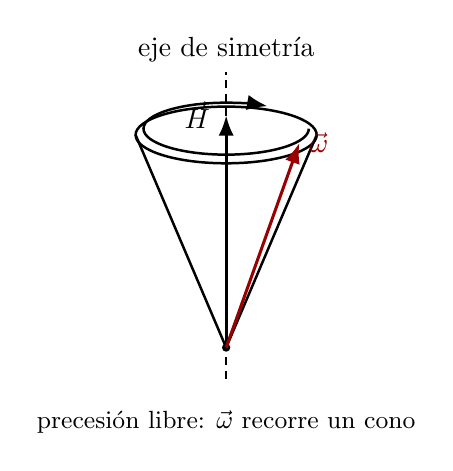
\begin{tikzpicture}[line width=0.9pt,>={Latex[length=2.6mm]}]
  \draw[densely dashed] (0,-0.4)--(0,3.5);
  \node[above] at (0,3.5){eje de simetría};
  % base del cono
  \draw (0,2.7) ellipse (1.15 and 0.36);
  \draw (0,0)--(1.15,2.7); \draw (0,0)--(-1.15,2.7);
  \fill (0,0) circle(1.5pt);
  % H a lo largo del eje
  \draw[->,line width=1.1pt] (0,0)--(0,2.95) node[left=2pt]{$\vec H$};
  % omega traza el cono
  \draw[->,red!60!black,line width=1.1pt] (0,0)--(0.93,2.6) node[right]{$\vec\omega$};
  % precesion sobre la elipse
  \draw[->] (1.05,2.78) arc (0:-300:1.05 and 0.33);
  \node at (0,-0.95){\small precesión libre: $\vec\omega$ recorre un cono};
\end{tikzpicture}
\end{document}
